\section{Quantum Computing}

	\begin{frame}[plain]
		\vfill
		\centering
		\begin{beamercolorbox}[sep=8pt,center,shadow=true,rounded=true]{title}
			\textbf{\usebeamerfont{title}\insertsectionhead}\par%
			\color{polimiblue}\noindent\rule{10cm}{1pt} \\
			\textbf{Quantum Computing Introduction}
		\end{beamercolorbox}
		\vfill
	\end{frame}

	\subsection{Quantum Physics}
		\begin{frame}{Quantum Physics}
			During the study of the state of the art of quantum computing we were able to define 8 important conclusions that we used in order to set the basis for the study of the SAT problem
			\begin{itemize}
				\item[1.] <1-> \textbf{Exponential growth of the state space}
				\item[2.] <2-> \textbf{Universal quantum computer is Turing complete}
				\item[3.] <3-> \textbf{State collapses after measurement}
				\item[4.] <4-> \textbf{No-cloning principle}
				\item[5.] <5-> \textbf{Uniform superposition of the initial state}
				\item[6.] <6-> \textbf{Can we solve $NP$-complete problems?}
				\item[7.] <7-> \textbf{Can we solve $NP$-hard problems?}
				\item[8.] <8-> \textbf{Query complexity}
			\end{itemize}
		\end{frame}
	
		\begin{frame}{Exponential growth of the state space}
			\small{\emph{The dimension of the state space of quantum registers grows exponentially in the number of qubits, whereas the dimension of the state space of classical registers grows linearly in the number of bits.\\}}
			
			\vspace{0.4cm}
			
			\begin{itemize}
				\item[$\bullet$] <1-> \textbf{Classical Register} \\
				Sequence of bits with values in $\{0,1\}$ \\
				The state of a classical machine with one register and n bits is a binary string in $\{0,1\}^n$ \\
				\textbf{Thus a n-dimensional space}
				
				\item[$\bullet$] <2-> \textbf{Quantum Register} \\
				Sequence of qubits with values in $[0,1]$ \\
				The state of a quantum machine with one register and n qubits is obtained by the tensor product of n $\mathbb{C}^2$ vectors \\
				\textbf{Thus a $2^n$ dimensional space}	
			\end{itemize}
		\end{frame}
	
		\begin{frame}{Universal quantum computer is Turing complete}
			\small
			\begin{center}
				\vspace{-1cm}
				\emph{A universal quantum computer is Turing-complete.}
			\end{center}
			A quantum register of n-qubits represents a quantum state $|\psi\rangle\in\mathbb{C}^{2^n}$.\\
			A quantum operation is a matrix $U$ such that:
			\begin{equation*}
				\centering
				U\in\mathbb{C}^{2^n\times 2^n}
			\end{equation*}
			The application of $U$ onto the state $|\psi\rangle$ is the unit vector:
			\begin{equation*}
				\centering
				U|\psi\rangle\in\mathbb{C}^{2^n}
			\end{equation*}
			The evolution of a state into another shows two important features of quantum gates:
			\begin{itemize}
				\item[1.] Quantum operations are \textbf{linear}
				\item[2.] Quantum operations are \textbf{reversible}
			\end{itemize}
			\textbf{It can be proved that a quantum machine with operations like $U$ is Turing complete}
		\end{frame}
	
		\begin{frame}{State collapses after measurement}
			\small
			\emph{The state of the quantum system after a measurement collapses to a linear combination of only those basis states that are consistent with the outcome of the measurement. The original quantum state is no longer recoverable.}
			
			\vspace{0.3cm}
			
			\begin{minipage}{0.6\textwidth}
				The \textbf{measurement} operation allows to bring on a classical bit the value of a qubit at the moment it is performed. Measuring a qubit is based on the famous quantum principles:
				\begin{itemize}
					\item[$\bullet$] Superposition
					\item[$\bullet$] Entanglement
				\end{itemize}
				It is typically used to measure the final state of a quantum machine to check if the expected result has been obtained
			\end{minipage}\hfill
			\begin{minipage}{0.4\textwidth}
				\centering
				\begin{figure}[h]
					\hspace{0.4cm}
					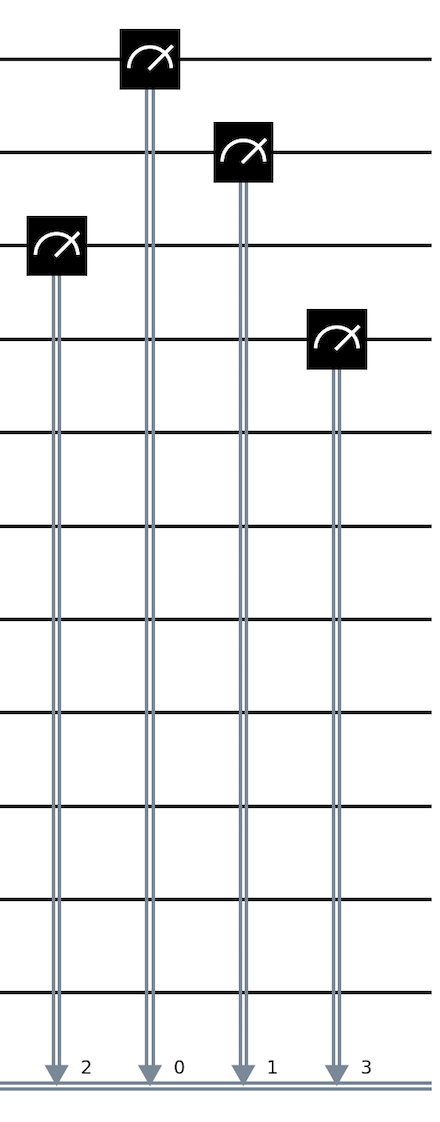
\includegraphics[scale=0.25]{measurementExample.png}
				\end{figure}
			\end{minipage}
		\end{frame}
	
		\begin{frame}{No-cloning principle}
			\small
			\begin{center}
				\vspace{-1cm}
				\emph{It is impossible to clone quantum states.}
			\end{center}
		
			\vspace{0.3cm}
		
			Measuring a state makes it collapse to a boring sequence of 1s and 0s\\
			A measured qubit is no longer in superposition, it is either 1 or 0 \\
			\begin{equation*}
				\underline{Is\;it\;possible\;to\;copy\;a\;state\;before\;measuring\;it\;?}
			\end{equation*}
			
			\vspace{0.3cm}
			
			The answer unfortunately is \textbf{NO!}\\
			It may be useful to split the execution of the quantum algorithm continuing with different operations on the same state
			
			\vspace{0.3cm}
			
			\textbf{Whenever we run a circuit that produces an output quantum state, in general we can reproduce the output quantum state by only repeating all the steps of the algorithm.}
		\end{frame}
	
		\begin{frame}{Uniform superposition of the initial state}
			\small
			\emph{Applying operations on a quantum device whose state is in a uniform superposition allows to apply them simultaneously to all possible binary strings thanks to linearity.}
			
			\vspace{0.3cm}
			
			To achieve the power of this conclusion we typically initialize the state of the quantum machine in a uniform superposition\\
			
			\vspace{0.2cm}
			
			The \textbf{Hadamard} gate on all the n-qubits of the register brings the initial state in the uniform superposition\\
			
			\vspace{0.2cm}
			
			We will see how to use it in the first step of \textbf{Grover's search algorithm}\\
			
			\vspace{0.2cm}
			
			The formal definition of an n-Hadamard gate is:
			\begin{equation*}
				\centering
				\bigotimes^{n}\mathcal{H} = \frac{1}{\sqrt{2}}
				\begin{pmatrix}
					\bigotimes^{n-1}\mathcal{H} & \bigotimes^{n-1}\mathcal{H} \\
					\bigotimes^{n-1}\mathcal{H} & -\bigotimes^{n-1}\mathcal{H}
				\end{pmatrix}
			\end{equation*}
		\end{frame}
	
		\begin{frame}{Can we solve $NP$ problems?}
			\small
			\textbf{Conclusion 6:\\}
			\emph{Even if we can easily create a uniform superposition of all basis states, the rules of measurement imply that using just this easily-obtained superposition does not allow us satisfactorily solve NP-complete problems, such as, for example, SAT.\\}
			\vspace{0.2cm}
			\textbf{Conclusion 7:\\}
			\emph{In general solving NP-Hard problems in polynomial time with quantum computers is not believed to be possible.}
			\vspace{0.3cm}
			\begin{figure}[h]
				\centering
				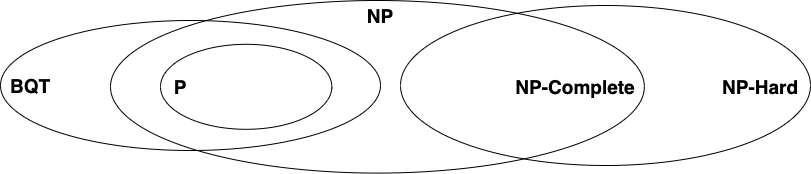
\includegraphics[scale=0.35]{problemsClassDiagram.png}
			\end{figure}
		\end{frame}
		
		\begin{frame}{Query complexity}
			\small
			\emph{The complexity of a quantum algorithm that belongs to the search class is determined only in terms of the number of the calls to the function f.}
			
			\vspace{0.3cm}
			
			Grover's algorithm is a search algorithm based on the call of a general function $f$\\
			
			\vspace{0.2cm}
			
			In quantum algorithms of this type we compute the \textbf{query complexity} rather than the number of elementary instructions executed by the program \\
			
			\vspace{0.2cm}
			
			Thanks to this different definition we will be able to describe through the 3 steps of Grover's search how a \textbf{quadratic} speedup is achieved w.r.t. a classical search algorithm
		\end{frame}
	
	\subsection{The Quantum Computer}
		\begin{frame}{The Quantum Computer}
			\small
			These conclusions allow to formally define the \emph{quantum machine paradigm} to be used in order to implement quantum algorithms
			\begin{figure}[h]
				\centering
				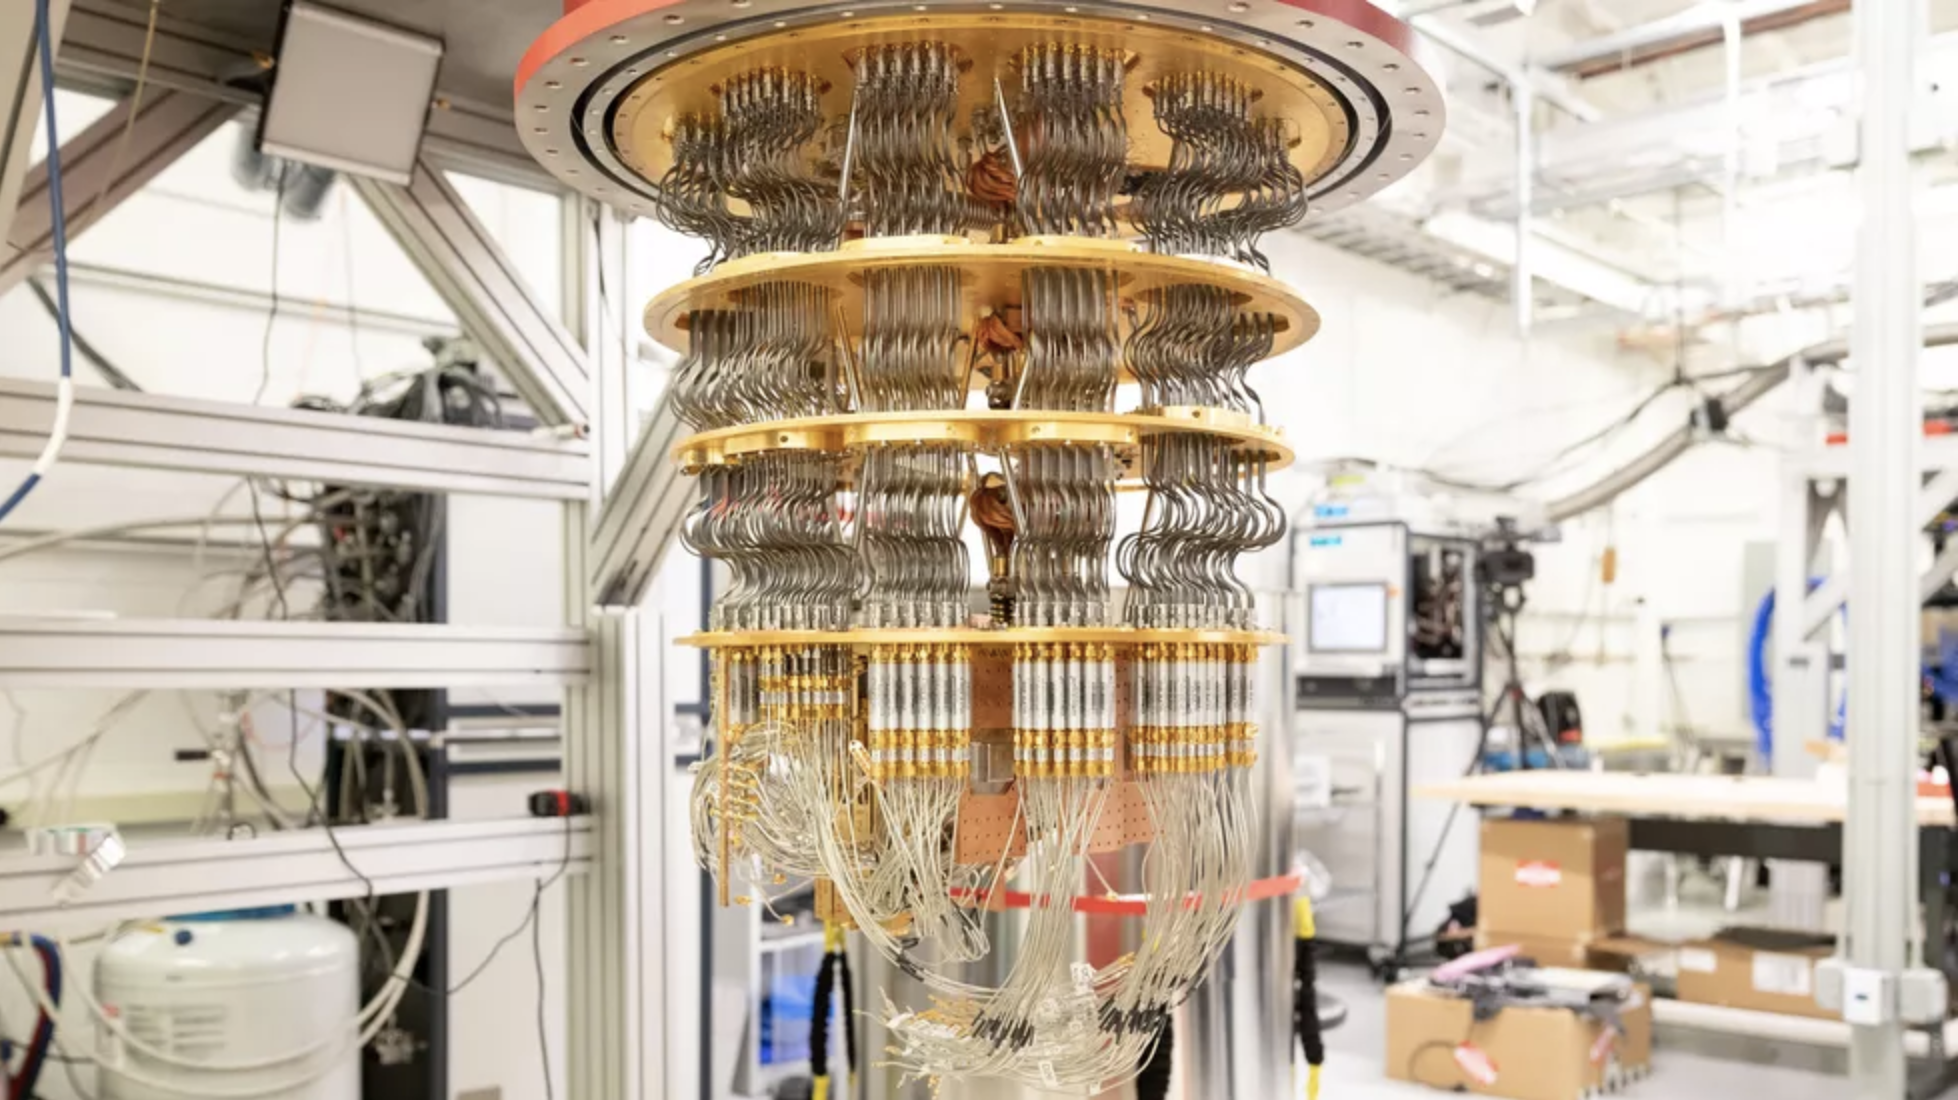
\includegraphics[scale=0.3]{googleQuantumComputer.png}
			\end{figure}
		\end{frame}
	
		\begin{frame}{The Quantum Computer Paradigm}
			A quantum computer is not that different from how we consider a classical one in a general point of view\\
			
			\vspace{0.3cm}
			
			The model of computation we considered to formalize this paradigm is the \textbf{quantum circuit model}, which works as follows:
			\begin{itemize}
				\item[$\bullet$] <1-> The quantum computer has a \textbf{state} that is stored in a quantum register, initialized in a certain way at the beginning of the computation
				
				\item[$\bullet$] <2-> \textbf{Quantum operations} applied on a state allow the quantum computer to evolve from a state to another
				
				\item[$\bullet$] <3-> At the end of the computation the information stored in the quantum register, thus the final state, contains the \textbf{result}
			\end{itemize}
		\end{frame}
	
	\subsection{Grover's Algorithm}
		\begin{frame}{Grover's Algorithm}
			\small
			Grover's algorithm is a search algorithm studied for database lookups based on the quantum principle called \textbf{Amplitude Amplification}\\
			
			\vspace{0.2cm}
			
			\textbf{Basic Idea:} \emph{Start with the uniform superposition of all basis states, and iteratively increase the coefficients of basis states that correspond to binary strings for which an unknown function gives output 1.}\\
			
			\vspace{0.3cm}
			
			The algorithm requires $q = n + 1$ qubits but we will need more to implement it in the generalized solver for the \textbf{exactly-1 k-SAT}\\
			
			\vspace{0.2cm}
			
			\textbf{Outline:} \emph{Obtained the uniform superposition of the quantum state the following steps are iteratively repeated:}
			\begin{itemize}
				\item[$\bullet$] Flip the sign of the vectors for which $U_f$ gives output 1
				\item[$\bullet$] Invert all the coefficients of the quantum state around the average coefficient
			\end{itemize}
		\end{frame}
	